\documentclass[twoside]{book}

% Packages required by doxygen
\usepackage{fixltx2e}
\usepackage{calc}
\usepackage{doxygen}
\usepackage[export]{adjustbox} % also loads graphicx
\usepackage{graphicx}
\usepackage[utf8]{inputenc}
\usepackage{makeidx}
\usepackage{multicol}
\usepackage{multirow}
\PassOptionsToPackage{warn}{textcomp}
\usepackage{textcomp}
\usepackage[nointegrals]{wasysym}
\usepackage[table]{xcolor}

% NLS support packages
\usepackage[spanish]{babel}
% Font selection
\usepackage[T1]{fontenc}
\usepackage[scaled=.90]{helvet}
\usepackage{courier}
\usepackage{amssymb}
\usepackage{sectsty}
\renewcommand{\familydefault}{\sfdefault}
\allsectionsfont{%
  \fontseries{bc}\selectfont%
  \color{darkgray}%
}
\renewcommand{\DoxyLabelFont}{%
  \fontseries{bc}\selectfont%
  \color{darkgray}%
}
\newcommand{\+}{\discretionary{\mbox{\scriptsize$\hookleftarrow$}}{}{}}

% Page & text layout
\usepackage{geometry}
\geometry{%
  a4paper,%
  top=2.5cm,%
  bottom=2.5cm,%
  left=2.5cm,%
  right=2.5cm%
}
\tolerance=750
\hfuzz=15pt
\hbadness=750
\setlength{\emergencystretch}{15pt}
\setlength{\parindent}{0cm}
\setlength{\parskip}{3ex plus 2ex minus 2ex}
\makeatletter
\renewcommand{\paragraph}{%
  \@startsection{paragraph}{4}{0ex}{-1.0ex}{1.0ex}{%
    \normalfont\normalsize\bfseries\SS@parafont%
  }%
}
\renewcommand{\subparagraph}{%
  \@startsection{subparagraph}{5}{0ex}{-1.0ex}{1.0ex}{%
    \normalfont\normalsize\bfseries\SS@subparafont%
  }%
}
\makeatother

% Headers & footers
\usepackage{fancyhdr}
\pagestyle{fancyplain}
\fancyhead[LE]{\fancyplain{}{\bfseries\thepage}}
\fancyhead[CE]{\fancyplain{}{}}
\fancyhead[RE]{\fancyplain{}{\bfseries\leftmark}}
\fancyhead[LO]{\fancyplain{}{\bfseries\rightmark}}
\fancyhead[CO]{\fancyplain{}{}}
\fancyhead[RO]{\fancyplain{}{\bfseries\thepage}}
\fancyfoot[LE]{\fancyplain{}{}}
\fancyfoot[CE]{\fancyplain{}{}}
\fancyfoot[RE]{\fancyplain{}{\bfseries\scriptsize Generado por Doxygen }}
\fancyfoot[LO]{\fancyplain{}{\bfseries\scriptsize Generado por Doxygen }}
\fancyfoot[CO]{\fancyplain{}{}}
\fancyfoot[RO]{\fancyplain{}{}}
\renewcommand{\footrulewidth}{0.4pt}
\renewcommand{\chaptermark}[1]{%
  \markboth{#1}{}%
}
\renewcommand{\sectionmark}[1]{%
  \markright{\thesection\ #1}%
}

% Indices & bibliography
\usepackage{natbib}
\usepackage[titles]{tocloft}
\setcounter{tocdepth}{3}
\setcounter{secnumdepth}{5}
\makeindex

% Hyperlinks (required, but should be loaded last)
\usepackage{ifpdf}
\ifpdf
  \usepackage[pdftex,pagebackref=true]{hyperref}
\else
  \usepackage[ps2pdf,pagebackref=true]{hyperref}
\fi
\hypersetup{%
  colorlinks=true,%
  linkcolor=blue,%
  citecolor=blue,%
  unicode%
}

% Custom commands
\newcommand{\clearemptydoublepage}{%
  \newpage{\pagestyle{empty}\cleardoublepage}%
}

\usepackage{caption}
\captionsetup{labelsep=space,justification=centering,font={bf},singlelinecheck=off,skip=4pt,position=top}

%===== C O N T E N T S =====

\begin{document}

% Titlepage & ToC
\hypersetup{pageanchor=false,
             bookmarksnumbered=true,
             pdfencoding=unicode
            }
\pagenumbering{alph}
\begin{titlepage}
\vspace*{7cm}
\begin{center}%
{\Large Laboratorio de P\+R\+O2. Ejercicio \textquotesingle{}Gestión de una lavadora\textquotesingle{}. \\[1ex]\large version 4 15-\/abr-\/2018 }\\
\vspace*{1cm}
{\large Generado por Doxygen 1.8.14}\\
\end{center}
\end{titlepage}
\clearemptydoublepage
\pagenumbering{roman}
\tableofcontents
\clearemptydoublepage
\pagenumbering{arabic}
\hypersetup{pageanchor=true}

%--- Begin generated contents ---
\chapter{Ejemplo de diseño modular\+: Gestión de una lavadora.}
\label{index}\hypertarget{index}{}En este ejemplo se construye un programa modular que ofrece un menú de opciones para gestionar una lavadora. Se introducen las clases {\itshape \mbox{\hyperlink{class_lavadora}{Lavadora}}}, {\itshape \mbox{\hyperlink{class_cubeta}{Cubeta}}} y {\itshape \mbox{\hyperlink{class_prenda}{Prenda}}}.

Sólo se documentan elementos públicos. En una próxima sesión se verá un ejemplo de proyecto completamente documentado, incluyendo los elementos privados. 
\chapter{Índice de clases}
\doxysection{Lista de clases}
Lista de las clases, estructuras, uniones e interfaces con una breve descripción\+:\begin{DoxyCompactList}
\item\contentsline{section}{\mbox{\hyperlink{class_alfabeto}{Alfabeto}} }{\pageref{class_alfabeto}}{}
\item\contentsline{section}{\mbox{\hyperlink{class_c_alfabetos}{C\+Alfabetos}} }{\pageref{class_c_alfabetos}}{}
\item\contentsline{section}{\mbox{\hyperlink{class_c_mensajes}{C\+Mensajes}} }{\pageref{class_c_mensajes}}{}
\item\contentsline{section}{\mbox{\hyperlink{class_mensaje}{Mensaje}} }{\pageref{class_mensaje}}{}
\end{DoxyCompactList}

\chapter{Indice de archivos}
\doxysection{Llista dels Fitxers}
Aquesta és la llista de tots els fitxers acompanyats amb breus descripcions\+:\begin{DoxyCompactList}
\item\contentsline{section}{\mbox{\hyperlink{_alfabeto_8hh}{Alfabeto.\+hh}} \\*Especificación de la clase alfabeto }{\pageref{_alfabeto_8hh}}{}
\item\contentsline{section}{\mbox{\hyperlink{_bin_tree_8hh}{Bin\+Tree.\+hh}} }{\pageref{_bin_tree_8hh}}{}
\item\contentsline{section}{\mbox{\hyperlink{_c_alfabetos_8hh}{C\+Alfabetos.\+hh}} \\*Especificación de la clase conjunto de alfabetos }{\pageref{_c_alfabetos_8hh}}{}
\item\contentsline{section}{\mbox{\hyperlink{_c_mensajes_8hh}{C\+Mensajes.\+hh}} \\*Especificación de la clase conjunto de mensajes }{\pageref{_c_mensajes_8hh}}{}
\item\contentsline{section}{\mbox{\hyperlink{_mensaje_8hh}{Mensaje.\+hh}} \\*Especificación de la clase mensaje }{\pageref{_mensaje_8hh}}{}
\item\contentsline{section}{\mbox{\hyperlink{_program_8cc}{Program.\+cc}} \\*Programa main }{\pageref{_program_8cc}}{}
\end{DoxyCompactList}

\chapter{Documentación de las clases}
\hypertarget{class_cubeta}{}\section{Referencia de la Clase Cubeta}
\label{class_cubeta}\index{Cubeta@{Cubeta}}


Representa una cubeta de ropa.  


\subsection*{Métodos públicos}
\begin{DoxyCompactItemize}
\item 
\mbox{\hyperlink{class_cubeta_ae85e70c9cd67454446439891e3f435e1}{Cubeta}} ()
\begin{DoxyCompactList}\small\item\em Creadora por defecto. \end{DoxyCompactList}\item 
\mbox{\hyperlink{class_cubeta_a9615e48038899c5732f61661585f12c7}{Cubeta}} (const \mbox{\hyperlink{class_cubeta}{Cubeta}} \&c)
\begin{DoxyCompactList}\small\item\em Creadora copiadora. \end{DoxyCompactList}\item 
void \mbox{\hyperlink{class_cubeta_a431873df8f99cebe56b4787a5271e395}{anadir\+\_\+prenda}} (const \mbox{\hyperlink{class_prenda}{Prenda}} \&p)
\begin{DoxyCompactList}\small\item\em Añade una prenda a la cubeta. \end{DoxyCompactList}\item 
void \mbox{\hyperlink{class_cubeta_a60a5a4f4133ce02f1e4fe49bbe8b9ec7}{completar\+\_\+lavadora}} (\mbox{\hyperlink{class_lavadora}{Lavadora}} \&lav)
\begin{DoxyCompactList}\small\item\em Completa una lavadora con las prendas de la cubeta. \end{DoxyCompactList}\item 
void \mbox{\hyperlink{class_cubeta_a3153ac390389f689bead058cd0b1690e}{escribir}} () const
\begin{DoxyCompactList}\small\item\em Operación de escritura. \end{DoxyCompactList}\end{DoxyCompactItemize}


\subsection{Descripción detallada}
Representa una cubeta de ropa. 

Puede contener prendas blancas y de color. Puede usarse para intentar llenar una lavadora; en ese caso, las prendas se sacan de la cubeta en orden inverso al de entrada 

Definición en la línea 21 del archivo Cubeta.\+hh.



\subsection{Documentación del constructor y destructor}
\mbox{\Hypertarget{class_cubeta_ae85e70c9cd67454446439891e3f435e1}\label{class_cubeta_ae85e70c9cd67454446439891e3f435e1}} 
\index{Cubeta@{Cubeta}!Cubeta@{Cubeta}}
\index{Cubeta@{Cubeta}!Cubeta@{Cubeta}}
\subsubsection{\texorpdfstring{Cubeta()}{Cubeta()}\hspace{0.1cm}{\footnotesize\ttfamily [1/2]}}
{\footnotesize\ttfamily Cubeta\+::\+Cubeta (\begin{DoxyParamCaption}{ }\end{DoxyParamCaption})}



Creadora por defecto. 

Se ejecuta automáticamente al declarar una cubeta. \begin{DoxyPrecond}{Precondición}
{\itshape cierto} 
\end{DoxyPrecond}
\begin{DoxyPostcond}{Postcondición}
El resultado es una cubeta sin prendas de ningún tipo 
\end{DoxyPostcond}
\begin{DoxyParagraph}{Coste Constante}

\end{DoxyParagraph}
\mbox{\Hypertarget{class_cubeta_a9615e48038899c5732f61661585f12c7}\label{class_cubeta_a9615e48038899c5732f61661585f12c7}} 
\index{Cubeta@{Cubeta}!Cubeta@{Cubeta}}
\index{Cubeta@{Cubeta}!Cubeta@{Cubeta}}
\subsubsection{\texorpdfstring{Cubeta()}{Cubeta()}\hspace{0.1cm}{\footnotesize\ttfamily [2/2]}}
{\footnotesize\ttfamily Cubeta\+::\+Cubeta (\begin{DoxyParamCaption}\item[{const \mbox{\hyperlink{class_cubeta}{Cubeta}} \&}]{c }\end{DoxyParamCaption})}



Creadora copiadora. 

Permite declarar una cubeta nueva como copia de otra ya existente. \begin{DoxyPrecond}{Precondición}
{\itshape cierto} 
\end{DoxyPrecond}
\begin{DoxyPostcond}{Postcondición}
El resultado es una cubeta igual que c 
\end{DoxyPostcond}
\begin{DoxyParagraph}{Coste Lineal respecto al número de prendas de c}

\end{DoxyParagraph}


\subsection{Documentación de las funciones miembro}
\mbox{\Hypertarget{class_cubeta_a431873df8f99cebe56b4787a5271e395}\label{class_cubeta_a431873df8f99cebe56b4787a5271e395}} 
\index{Cubeta@{Cubeta}!anadir\+\_\+prenda@{anadir\+\_\+prenda}}
\index{anadir\+\_\+prenda@{anadir\+\_\+prenda}!Cubeta@{Cubeta}}
\subsubsection{\texorpdfstring{anadir\+\_\+prenda()}{anadir\_prenda()}}
{\footnotesize\ttfamily void Cubeta\+::anadir\+\_\+prenda (\begin{DoxyParamCaption}\item[{const \mbox{\hyperlink{class_prenda}{Prenda}} \&}]{p }\end{DoxyParamCaption})}



Añade una prenda a la cubeta. 

\begin{DoxyPrecond}{Precondición}
{\itshape cierto} 
\end{DoxyPrecond}
\begin{DoxyPostcond}{Postcondición}
El parámetro implícito pasa a contener sus prendas originales más p 
\end{DoxyPostcond}
\begin{DoxyParagraph}{Coste Constante}

\end{DoxyParagraph}
\mbox{\Hypertarget{class_cubeta_a60a5a4f4133ce02f1e4fe49bbe8b9ec7}\label{class_cubeta_a60a5a4f4133ce02f1e4fe49bbe8b9ec7}} 
\index{Cubeta@{Cubeta}!completar\+\_\+lavadora@{completar\+\_\+lavadora}}
\index{completar\+\_\+lavadora@{completar\+\_\+lavadora}!Cubeta@{Cubeta}}
\subsubsection{\texorpdfstring{completar\+\_\+lavadora()}{completar\_lavadora()}}
{\footnotesize\ttfamily void Cubeta\+::completar\+\_\+lavadora (\begin{DoxyParamCaption}\item[{\mbox{\hyperlink{class_lavadora}{Lavadora}} \&}]{lav }\end{DoxyParamCaption})}



Completa una lavadora con las prendas de la cubeta. 

\begin{DoxyPrecond}{Precondición}
lav está inicializada 
\end{DoxyPrecond}
\begin{DoxyPostcond}{Postcondición}
Se han eliminado del parámetro implícito y se han añadido a lav las prendas del parámetro implícito del color adecuado que más se acercan entre todas al peso máximo de lav sin pasarse, elegiéndose primero las que se introdujeron en último lugar 
\end{DoxyPostcond}
\begin{DoxyParagraph}{Coste Lineal respecto al número de prendas del parámetro implícito }

\end{DoxyParagraph}
\mbox{\Hypertarget{class_cubeta_a3153ac390389f689bead058cd0b1690e}\label{class_cubeta_a3153ac390389f689bead058cd0b1690e}} 
\index{Cubeta@{Cubeta}!escribir@{escribir}}
\index{escribir@{escribir}!Cubeta@{Cubeta}}
\subsubsection{\texorpdfstring{escribir()}{escribir()}}
{\footnotesize\ttfamily void Cubeta\+::escribir (\begin{DoxyParamCaption}{ }\end{DoxyParamCaption}) const}



Operación de escritura. 

\begin{DoxyPrecond}{Precondición}
{\itshape cierto} 
\end{DoxyPrecond}
\begin{DoxyPostcond}{Postcondición}
Escribe el contenido del parámetro implícito por el canal estándar de salida 
\end{DoxyPostcond}
\begin{DoxyParagraph}{Coste Lineal respecto al número de prendas del parámetro implícito }

\end{DoxyParagraph}


La documentación para esta clase fue generada a partir del siguiente fichero\+:\begin{DoxyCompactItemize}
\item 
\mbox{\hyperlink{_cubeta_8hh}{Cubeta.\+hh}}\end{DoxyCompactItemize}

\hypertarget{class_lavadora}{}\section{Referencia de la Clase Lavadora}
\label{class_lavadora}\index{Lavadora@{Lavadora}}


Representa una lavadora.  


\subsection*{Métodos públicos}
\begin{DoxyCompactItemize}
\item 
\mbox{\hyperlink{class_lavadora_a2366b1cd0ba86f8ef8ba8504067dc114}{Lavadora}} ()
\begin{DoxyCompactList}\small\item\em Creadora por defecto. \end{DoxyCompactList}\item 
void \mbox{\hyperlink{class_lavadora_a733af02910dca3f75390be4ca6ac84f6}{inicializar}} (int pmax, bool col)
\begin{DoxyCompactList}\small\item\em Inicializa la lavadora. \end{DoxyCompactList}\item 
void \mbox{\hyperlink{class_lavadora_a7e465e1f11ba5ba3cffcee1ce9507e79}{anadir\+\_\+prenda}} (const \mbox{\hyperlink{class_prenda}{Prenda}} \&p)
\begin{DoxyCompactList}\small\item\em Añade una prenda a la lavadora. \end{DoxyCompactList}\item 
void \mbox{\hyperlink{class_lavadora_a82bd403e688482030fcb95f0c3fd62d1}{lavado}} ()
\begin{DoxyCompactList}\small\item\em Realiza un lavado. \end{DoxyCompactList}\item 
bool \mbox{\hyperlink{class_lavadora_af081f8133ddfca2fd4f1f79575620c5a}{esta\+\_\+inicializada}} () const
\begin{DoxyCompactList}\small\item\em Consultora del estado de la lavadora. \end{DoxyCompactList}\item 
bool \mbox{\hyperlink{class_lavadora_a5d538cc8efce89e5da5a38d879bb2659}{consultar\+\_\+color}} () const
\begin{DoxyCompactList}\small\item\em Consultora del color de la lavadora. \end{DoxyCompactList}\item 
int \mbox{\hyperlink{class_lavadora_a411751a432a84ab91196e6b827190f05}{consultar\+\_\+peso}} () const
\begin{DoxyCompactList}\small\item\em Consultora del peso actual de la lavadora. \end{DoxyCompactList}\item 
int \mbox{\hyperlink{class_lavadora_a725ef6a2786b400e0cffebe7a690602e}{consultar\+\_\+peso\+\_\+maximo}} () const
\begin{DoxyCompactList}\small\item\em Consultora del peso máximo de la lavadora. \end{DoxyCompactList}\item 
void \mbox{\hyperlink{class_lavadora_a2372c33a5f76dda6e3892d118ae726f1}{escribir}} () const
\begin{DoxyCompactList}\small\item\em Operación de escritura. \end{DoxyCompactList}\end{DoxyCompactItemize}


\subsection{Descripción detallada}
Representa una lavadora. 

Dispone de dos estados posibles (inicializada / no inicializada); si está inicializada tiene un peso máximo y un color y puede contener prendas de dicho color hasta alcanzar dicho peso máximo; si no está inicializada no contiene ninguna prenda y solo se puede inicializar

Todas las operaciones son de {\bfseries coste constante} salvo las indicadas 

Definición en la línea 20 del archivo Lavadora.\+hh.



\subsection{Documentación del constructor y destructor}
\mbox{\Hypertarget{class_lavadora_a2366b1cd0ba86f8ef8ba8504067dc114}\label{class_lavadora_a2366b1cd0ba86f8ef8ba8504067dc114}} 
\index{Lavadora@{Lavadora}!Lavadora@{Lavadora}}
\index{Lavadora@{Lavadora}!Lavadora@{Lavadora}}
\subsubsection{\texorpdfstring{Lavadora()}{Lavadora()}}
{\footnotesize\ttfamily Lavadora\+::\+Lavadora (\begin{DoxyParamCaption}{ }\end{DoxyParamCaption})}



Creadora por defecto. 

Se ejecuta automáticamente al declarar una lavadora. \begin{DoxyPrecond}{Precondición}
{\itshape cierto} 
\end{DoxyPrecond}
\begin{DoxyPostcond}{Postcondición}
El resultado es una lavadora no inicializada 
\end{DoxyPostcond}


\subsection{Documentación de las funciones miembro}
\mbox{\Hypertarget{class_lavadora_a733af02910dca3f75390be4ca6ac84f6}\label{class_lavadora_a733af02910dca3f75390be4ca6ac84f6}} 
\index{Lavadora@{Lavadora}!inicializar@{inicializar}}
\index{inicializar@{inicializar}!Lavadora@{Lavadora}}
\subsubsection{\texorpdfstring{inicializar()}{inicializar()}}
{\footnotesize\ttfamily void Lavadora\+::inicializar (\begin{DoxyParamCaption}\item[{int}]{pmax,  }\item[{bool}]{col }\end{DoxyParamCaption})}



Inicializa la lavadora. 

\begin{DoxyPrecond}{Precondición}
El parámetro implícito no está inicializado, pmax$>$0 
\end{DoxyPrecond}
\begin{DoxyPostcond}{Postcondición}
El parámetro implícito pasa a estar inicializado con peso máximo \char`\"{}pmax\char`\"{} y color \char`\"{}col\char`\"{} 
\end{DoxyPostcond}
\mbox{\Hypertarget{class_lavadora_a7e465e1f11ba5ba3cffcee1ce9507e79}\label{class_lavadora_a7e465e1f11ba5ba3cffcee1ce9507e79}} 
\index{Lavadora@{Lavadora}!anadir\+\_\+prenda@{anadir\+\_\+prenda}}
\index{anadir\+\_\+prenda@{anadir\+\_\+prenda}!Lavadora@{Lavadora}}
\subsubsection{\texorpdfstring{anadir\+\_\+prenda()}{anadir\_prenda()}}
{\footnotesize\ttfamily void Lavadora\+::anadir\+\_\+prenda (\begin{DoxyParamCaption}\item[{const \mbox{\hyperlink{class_prenda}{Prenda}} \&}]{p }\end{DoxyParamCaption})}



Añade una prenda a la lavadora. 

\begin{DoxyPrecond}{Precondición}
El parámetro implícito (L) está inicializado, color de p = color de L, peso de L + peso de p $<$= peso máximo de L 
\end{DoxyPrecond}
\begin{DoxyPostcond}{Postcondición}
El parámetro implícito contiene su carga original más p 
\end{DoxyPostcond}
\mbox{\Hypertarget{class_lavadora_a82bd403e688482030fcb95f0c3fd62d1}\label{class_lavadora_a82bd403e688482030fcb95f0c3fd62d1}} 
\index{Lavadora@{Lavadora}!lavado@{lavado}}
\index{lavado@{lavado}!Lavadora@{Lavadora}}
\subsubsection{\texorpdfstring{lavado()}{lavado()}}
{\footnotesize\ttfamily void Lavadora\+::lavado (\begin{DoxyParamCaption}{ }\end{DoxyParamCaption})}



Realiza un lavado. 

Representa que se realiza el lavado, se retiran la prendas que contiene la lavadora y ésta queda en estado de volver a usarse \begin{DoxyPrecond}{Precondición}
El parámetro implícito está inicializado 
\end{DoxyPrecond}
\begin{DoxyPostcond}{Postcondición}
El parámetro implícito no está inicializado 
\end{DoxyPostcond}
\begin{DoxyParagraph}{Coste Lineal respecto al número de prendas del parámetro implícito}

\end{DoxyParagraph}
\mbox{\Hypertarget{class_lavadora_af081f8133ddfca2fd4f1f79575620c5a}\label{class_lavadora_af081f8133ddfca2fd4f1f79575620c5a}} 
\index{Lavadora@{Lavadora}!esta\+\_\+inicializada@{esta\+\_\+inicializada}}
\index{esta\+\_\+inicializada@{esta\+\_\+inicializada}!Lavadora@{Lavadora}}
\subsubsection{\texorpdfstring{esta\+\_\+inicializada()}{esta\_inicializada()}}
{\footnotesize\ttfamily bool Lavadora\+::esta\+\_\+inicializada (\begin{DoxyParamCaption}{ }\end{DoxyParamCaption}) const}



Consultora del estado de la lavadora. 

\begin{DoxyPrecond}{Precondición}
{\itshape cierto} 
\end{DoxyPrecond}
\begin{DoxyPostcond}{Postcondición}
El resultado indica si el parámetro implícito está inicializado 
\end{DoxyPostcond}
\mbox{\Hypertarget{class_lavadora_a5d538cc8efce89e5da5a38d879bb2659}\label{class_lavadora_a5d538cc8efce89e5da5a38d879bb2659}} 
\index{Lavadora@{Lavadora}!consultar\+\_\+color@{consultar\+\_\+color}}
\index{consultar\+\_\+color@{consultar\+\_\+color}!Lavadora@{Lavadora}}
\subsubsection{\texorpdfstring{consultar\+\_\+color()}{consultar\_color()}}
{\footnotesize\ttfamily bool Lavadora\+::consultar\+\_\+color (\begin{DoxyParamCaption}{ }\end{DoxyParamCaption}) const}



Consultora del color de la lavadora. 

\begin{DoxyPrecond}{Precondición}
El parámetro implícito está inicializado 
\end{DoxyPrecond}
\begin{DoxyPostcond}{Postcondición}
El resultado es el color del parámetro implícito 
\end{DoxyPostcond}
\mbox{\Hypertarget{class_lavadora_a411751a432a84ab91196e6b827190f05}\label{class_lavadora_a411751a432a84ab91196e6b827190f05}} 
\index{Lavadora@{Lavadora}!consultar\+\_\+peso@{consultar\+\_\+peso}}
\index{consultar\+\_\+peso@{consultar\+\_\+peso}!Lavadora@{Lavadora}}
\subsubsection{\texorpdfstring{consultar\+\_\+peso()}{consultar\_peso()}}
{\footnotesize\ttfamily int Lavadora\+::consultar\+\_\+peso (\begin{DoxyParamCaption}{ }\end{DoxyParamCaption}) const}



Consultora del peso actual de la lavadora. 

\begin{DoxyPrecond}{Precondición}
El parámetro implícito está inicializado 
\end{DoxyPrecond}
\begin{DoxyPostcond}{Postcondición}
El resultado es la suma de los pesos de las prendas del parámetro implícito 
\end{DoxyPostcond}
\mbox{\Hypertarget{class_lavadora_a725ef6a2786b400e0cffebe7a690602e}\label{class_lavadora_a725ef6a2786b400e0cffebe7a690602e}} 
\index{Lavadora@{Lavadora}!consultar\+\_\+peso\+\_\+maximo@{consultar\+\_\+peso\+\_\+maximo}}
\index{consultar\+\_\+peso\+\_\+maximo@{consultar\+\_\+peso\+\_\+maximo}!Lavadora@{Lavadora}}
\subsubsection{\texorpdfstring{consultar\+\_\+peso\+\_\+maximo()}{consultar\_peso\_maximo()}}
{\footnotesize\ttfamily int Lavadora\+::consultar\+\_\+peso\+\_\+maximo (\begin{DoxyParamCaption}{ }\end{DoxyParamCaption}) const}



Consultora del peso máximo de la lavadora. 

\begin{DoxyPrecond}{Precondición}
El parámetro implícito está inicializado 
\end{DoxyPrecond}
\begin{DoxyPostcond}{Postcondición}
El resultado es el peso máximo del parámetro implícito 
\end{DoxyPostcond}
\mbox{\Hypertarget{class_lavadora_a2372c33a5f76dda6e3892d118ae726f1}\label{class_lavadora_a2372c33a5f76dda6e3892d118ae726f1}} 
\index{Lavadora@{Lavadora}!escribir@{escribir}}
\index{escribir@{escribir}!Lavadora@{Lavadora}}
\subsubsection{\texorpdfstring{escribir()}{escribir()}}
{\footnotesize\ttfamily void Lavadora\+::escribir (\begin{DoxyParamCaption}{ }\end{DoxyParamCaption}) const}



Operación de escritura. 

\begin{DoxyPrecond}{Precondición}
El parámetro implícito está inicializado 
\end{DoxyPrecond}
\begin{DoxyPostcond}{Postcondición}
Escribe las propiedades y el contenido del parámetro implícito por el canal estándar de salida 
\end{DoxyPostcond}
\begin{DoxyParagraph}{Coste Lineal respecto al número de prendas del parámetro implícito}

\end{DoxyParagraph}


La documentación para esta clase fue generada a partir del siguiente fichero\+:\begin{DoxyCompactItemize}
\item 
\mbox{\hyperlink{_lavadora_8hh}{Lavadora.\+hh}}\end{DoxyCompactItemize}

\hypertarget{class_prenda}{}\section{Referencia de la Clase Prenda}
\label{class_prenda}\index{Prenda@{Prenda}}


Representa una prenda de ropa con atributos peso y color.  


\subsection*{Métodos públicos}
\begin{DoxyCompactItemize}
\item 
\mbox{\hyperlink{class_prenda_adfd86b131c7f40c58b0cb4200eb55129}{Prenda}} ()
\begin{DoxyCompactList}\small\item\em Creadora por defecto. \end{DoxyCompactList}\item 
\mbox{\hyperlink{class_prenda_af15ff723083040b89bc495b4ec4b914e}{Prenda}} (int pes, bool col)
\begin{DoxyCompactList}\small\item\em Creadora con valores concretos. \end{DoxyCompactList}\item 
void \mbox{\hyperlink{class_prenda_ab25b2a66034eb2c0fccfb1f3cedbb5a7}{modificar}} (int pes, bool col)
\begin{DoxyCompactList}\small\item\em Modificadora de los atributos. \end{DoxyCompactList}\item 
int \mbox{\hyperlink{class_prenda_aef786876c5b4bb4f8f7fdd980f332b14}{consul\+\_\+peso}} () const
\begin{DoxyCompactList}\small\item\em Consultora del peso. \end{DoxyCompactList}\item 
bool \mbox{\hyperlink{class_prenda_a81575030ecbaabf350091f54612033f4}{consul\+\_\+color}} () const
\begin{DoxyCompactList}\small\item\em Consultora del color. \end{DoxyCompactList}\item 
void \mbox{\hyperlink{class_prenda_a6261b483bb78e47266e353fdd11c3077}{escribir}} () const
\begin{DoxyCompactList}\small\item\em Operación de escritura. \end{DoxyCompactList}\end{DoxyCompactItemize}


\subsection{Descripción detallada}
Representa una prenda de ropa con atributos peso y color. 

Todas las operaciones son de {\bfseries coste constante} 

Definición en la línea 19 del archivo Prenda.\+hh.



\subsection{Documentación del constructor y destructor}
\mbox{\Hypertarget{class_prenda_adfd86b131c7f40c58b0cb4200eb55129}\label{class_prenda_adfd86b131c7f40c58b0cb4200eb55129}} 
\index{Prenda@{Prenda}!Prenda@{Prenda}}
\index{Prenda@{Prenda}!Prenda@{Prenda}}
\subsubsection{\texorpdfstring{Prenda()}{Prenda()}\hspace{0.1cm}{\footnotesize\ttfamily [1/2]}}
{\footnotesize\ttfamily Prenda\+::\+Prenda (\begin{DoxyParamCaption}{ }\end{DoxyParamCaption})}



Creadora por defecto. 

Se ejecuta automáticamente al declarar una prenda. \begin{DoxyPrecond}{Precondición}
{\itshape cierto} 
\end{DoxyPrecond}
\begin{DoxyPostcond}{Postcondición}
El resultado es una prenda de peso 0 y color blanco 
\end{DoxyPostcond}
\mbox{\Hypertarget{class_prenda_af15ff723083040b89bc495b4ec4b914e}\label{class_prenda_af15ff723083040b89bc495b4ec4b914e}} 
\index{Prenda@{Prenda}!Prenda@{Prenda}}
\index{Prenda@{Prenda}!Prenda@{Prenda}}
\subsubsection{\texorpdfstring{Prenda()}{Prenda()}\hspace{0.1cm}{\footnotesize\ttfamily [2/2]}}
{\footnotesize\ttfamily Prenda\+::\+Prenda (\begin{DoxyParamCaption}\item[{int}]{pes,  }\item[{bool}]{col }\end{DoxyParamCaption})}



Creadora con valores concretos. 

\begin{DoxyPrecond}{Precondición}
pes$>$0 
\end{DoxyPrecond}
\begin{DoxyPostcond}{Postcondición}
El resultado es una prenda con peso \char`\"{}pes\char`\"{} y color \char`\"{}col\char`\"{} 
\end{DoxyPostcond}


\subsection{Documentación de las funciones miembro}
\mbox{\Hypertarget{class_prenda_ab25b2a66034eb2c0fccfb1f3cedbb5a7}\label{class_prenda_ab25b2a66034eb2c0fccfb1f3cedbb5a7}} 
\index{Prenda@{Prenda}!modificar@{modificar}}
\index{modificar@{modificar}!Prenda@{Prenda}}
\subsubsection{\texorpdfstring{modificar()}{modificar()}}
{\footnotesize\ttfamily void Prenda\+::modificar (\begin{DoxyParamCaption}\item[{int}]{pes,  }\item[{bool}]{col }\end{DoxyParamCaption})}



Modificadora de los atributos. 

\begin{DoxyPrecond}{Precondición}
pes$>$0 
\end{DoxyPrecond}
\begin{DoxyPostcond}{Postcondición}
El parámetro implícito pasa a tener peso \char`\"{}pes\char`\"{} y color \char`\"{}col\char`\"{} 
\end{DoxyPostcond}
\mbox{\Hypertarget{class_prenda_aef786876c5b4bb4f8f7fdd980f332b14}\label{class_prenda_aef786876c5b4bb4f8f7fdd980f332b14}} 
\index{Prenda@{Prenda}!consul\+\_\+peso@{consul\+\_\+peso}}
\index{consul\+\_\+peso@{consul\+\_\+peso}!Prenda@{Prenda}}
\subsubsection{\texorpdfstring{consul\+\_\+peso()}{consul\_peso()}}
{\footnotesize\ttfamily int Prenda\+::consul\+\_\+peso (\begin{DoxyParamCaption}{ }\end{DoxyParamCaption}) const}



Consultora del peso. 

\begin{DoxyPrecond}{Precondición}
{\itshape cierto} 
\end{DoxyPrecond}
\begin{DoxyPostcond}{Postcondición}
El resultado es el peso del parámetro implícito 
\end{DoxyPostcond}
\mbox{\Hypertarget{class_prenda_a81575030ecbaabf350091f54612033f4}\label{class_prenda_a81575030ecbaabf350091f54612033f4}} 
\index{Prenda@{Prenda}!consul\+\_\+color@{consul\+\_\+color}}
\index{consul\+\_\+color@{consul\+\_\+color}!Prenda@{Prenda}}
\subsubsection{\texorpdfstring{consul\+\_\+color()}{consul\_color()}}
{\footnotesize\ttfamily bool Prenda\+::consul\+\_\+color (\begin{DoxyParamCaption}{ }\end{DoxyParamCaption}) const}



Consultora del color. 

\begin{DoxyPrecond}{Precondición}
{\itshape cierto} 
\end{DoxyPrecond}
\begin{DoxyPostcond}{Postcondición}
El resultado es el color del parámetro implícito 
\end{DoxyPostcond}
\mbox{\Hypertarget{class_prenda_a6261b483bb78e47266e353fdd11c3077}\label{class_prenda_a6261b483bb78e47266e353fdd11c3077}} 
\index{Prenda@{Prenda}!escribir@{escribir}}
\index{escribir@{escribir}!Prenda@{Prenda}}
\subsubsection{\texorpdfstring{escribir()}{escribir()}}
{\footnotesize\ttfamily void Prenda\+::escribir (\begin{DoxyParamCaption}{ }\end{DoxyParamCaption}) const}



Operación de escritura. 

\begin{DoxyPrecond}{Precondición}
{\itshape cierto} 
\end{DoxyPrecond}
\begin{DoxyPostcond}{Postcondición}
Se han escrito los atributos del parámetro implícito en el canal standard de salida. 
\end{DoxyPostcond}


La documentación para esta clase fue generada a partir del siguiente fichero\+:\begin{DoxyCompactItemize}
\item 
\mbox{\hyperlink{_prenda_8hh}{Prenda.\+hh}}\end{DoxyCompactItemize}

\chapter{Documentación de archivos}
\hypertarget{_cubeta_8hh}{}\section{Referencia del Archivo Cubeta.\+hh}
\label{_cubeta_8hh}\index{Cubeta.\+hh@{Cubeta.\+hh}}


Especificación de la clase \mbox{\hyperlink{class_cubeta}{Cubeta}}.  


Dependencia gráfica adjunta para Cubeta.\+hh\+:\nopagebreak
\begin{figure}[H]
\begin{center}
\leavevmode
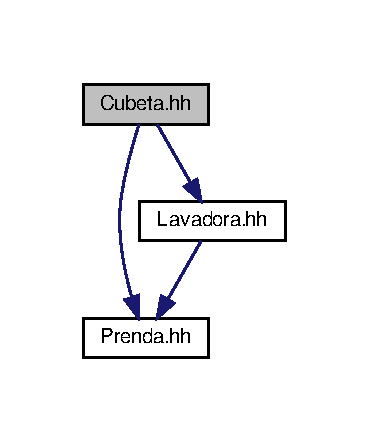
\includegraphics[width=177pt]{_cubeta_8hh__incl}
\end{center}
\end{figure}
\subsection*{Clases}
\begin{DoxyCompactItemize}
\item 
class \mbox{\hyperlink{class_cubeta}{Cubeta}}
\begin{DoxyCompactList}\small\item\em Representa una cubeta de ropa. \end{DoxyCompactList}\end{DoxyCompactItemize}


\subsection{Descripción detallada}
Especificación de la clase \mbox{\hyperlink{class_cubeta}{Cubeta}}. 


\hypertarget{_lavadora_8hh}{}\section{Referencia del Archivo Lavadora.\+hh}
\label{_lavadora_8hh}\index{Lavadora.\+hh@{Lavadora.\+hh}}


Especificación de la clase \mbox{\hyperlink{class_lavadora}{Lavadora}}.  


Dependencia gráfica adjunta para Lavadora.\+hh\+:\nopagebreak
\begin{figure}[H]
\begin{center}
\leavevmode
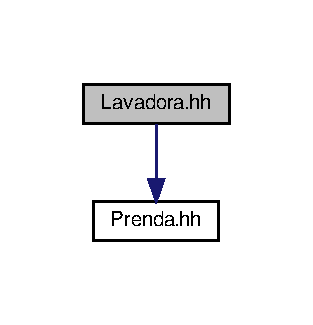
\includegraphics[width=150pt]{_lavadora_8hh__incl}
\end{center}
\end{figure}
\subsection*{Clases}
\begin{DoxyCompactItemize}
\item 
class \mbox{\hyperlink{class_lavadora}{Lavadora}}
\begin{DoxyCompactList}\small\item\em Representa una lavadora. \end{DoxyCompactList}\end{DoxyCompactItemize}


\subsection{Descripción detallada}
Especificación de la clase \mbox{\hyperlink{class_lavadora}{Lavadora}}. 


\hypertarget{_prenda_8hh}{}\section{Referencia del Archivo Prenda.\+hh}
\label{_prenda_8hh}\index{Prenda.\+hh@{Prenda.\+hh}}


Especificación de la clase \mbox{\hyperlink{class_prenda}{Prenda}}.  


\subsection*{Clases}
\begin{DoxyCompactItemize}
\item 
class \mbox{\hyperlink{class_prenda}{Prenda}}
\begin{DoxyCompactList}\small\item\em Representa una prenda de ropa con atributos peso y color. \end{DoxyCompactList}\end{DoxyCompactItemize}


\subsection{Descripción detallada}
Especificación de la clase \mbox{\hyperlink{class_prenda}{Prenda}}. 


\hypertarget{pro2__especif_8cc}{}\section{Referencia del Archivo pro2\+\_\+especif.\+cc}
\label{pro2__especif_8cc}\index{pro2\+\_\+especif.\+cc@{pro2\+\_\+especif.\+cc}}
Dependencia gráfica adjunta para pro2\+\_\+especif.\+cc\+:\nopagebreak
\begin{figure}[H]
\begin{center}
\leavevmode
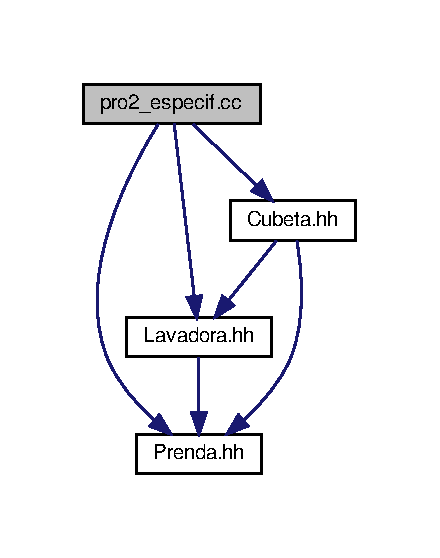
\includegraphics[width=211pt]{pro2__especif_8cc__incl}
\end{center}
\end{figure}
\subsection*{Funciones}
\begin{DoxyCompactItemize}
\item 
int \mbox{\hyperlink{pro2__especif_8cc_ae66f6b31b5ad750f1fe042a706a4e3d4}{main}} ()
\begin{DoxyCompactList}\small\item\em Programa principal para el ejercicio {\itshape Gestión de una lavadora}. \end{DoxyCompactList}\end{DoxyCompactItemize}


\subsection{Documentación de las funciones}
\mbox{\Hypertarget{pro2__especif_8cc_ae66f6b31b5ad750f1fe042a706a4e3d4}\label{pro2__especif_8cc_ae66f6b31b5ad750f1fe042a706a4e3d4}} 
\index{pro2\+\_\+especif.\+cc@{pro2\+\_\+especif.\+cc}!main@{main}}
\index{main@{main}!pro2\+\_\+especif.\+cc@{pro2\+\_\+especif.\+cc}}
\subsubsection{\texorpdfstring{main()}{main()}}
{\footnotesize\ttfamily int main (\begin{DoxyParamCaption}{ }\end{DoxyParamCaption})}



Programa principal para el ejercicio {\itshape Gestión de una lavadora}. 



Definición en la línea 25 del archivo pro2\+\_\+especif.\+cc.


\begin{DoxyCode}
26 \{
27 
28 \}
\end{DoxyCode}

%--- End generated contents ---

% Index
\backmatter
\newpage
\phantomsection
\clearemptydoublepage
\addcontentsline{toc}{chapter}{Índice}
\printindex

\end{document}
